\documentclass[11pt]{article}
\usepackage[margin=0.9in]{geometry}
\usepackage{amsmath,amssymb,graphicx,booktabs,hyperref,xcolor,float}
\usepackage[T1]{fontenc}
\graphicspath{{../v3s/}{../v3s/S2/}{../v3/}{../cocoa/analysis/}}
\newcommand{\hmpc}{\,h\,\mathrm{Mpc}^{-1}}
\newcommand{\dchi}{\Delta\chi^2}
\title{Scale cuts with the stitched FLAMINGO spectra as the truth\\[2pt]\large NLA / TATT goodness of fit, $\dchi$, cuts, amplitudes and the Roman figure of bias (companion to the 7 Nov summary)}
\author{Yijie Zhu, with Claude}
\date{7 November 2026}

\begin{document}
\maketitle

\section*{Summary}

This companion repeats the $k_{\max}$ analysis of the main summary (goodness
of fit, $\dchi^2_{\rm FL}$, redshift-dependent cuts, $A_1(z)$, $A_2(z)$,
translation to Roman, figure of bias) with the \emph{stitched} spectra of the
FLAMINGO notes as the truth: NLA fitted on large scales, the FLAMINGO spline on
small scales, joined by a logistic weight at $k_t(z)$. Section 7 adds the
Roman test with all parameters free on the same truth.

\begin{itemize}
\item \textbf{Cuts (core snapshots $0.2 \le z \le 2$, refit GoF, $p<0.05$).}
  NLA 0.22$\hmpc$ at $z \le 0.5$, 0.29 at $z = 0.6$, 0.39 at $z$ = 0.75 to
  1.5, 0.29 at $z = 2$; TATT 0.29 at $z \le 0.5$, 0.39 at $z$ = 0.6 to 1,
  0.52 at $z \ge 1.5$. Combined over the core: NLA fails at 0.29, TATT at
  0.39. The NLA cut sits at 1.1 to 1.9 times $k_t(z)$, i.e.\ the NLA fit
  survives about half a logistic width past the point where the simulation
  takes over. On the production truth (same two probes) the cuts are
  0.09 to 0.16 (NLA) and 0.22 to 0.52 (TATT).
\item \textbf{Fractional deviation of the anchored model from the truth.}
  Within 5 per cent on both GI and II: NLA 0.12 to 0.39, TATT 0.16 to 0.29;
  within 10 per cent: NLA 0.29 to 0.52, TATT 0.22 to 0.52.
\item \textbf{$\dchi^2_{\rm FL}$} (refit against the noise-free truth, core
  sum) at $k_{\max}$ = 0.22 / 0.29 / 0.39: NLA 9 / 50 / 327, TATT 9 / 30 /
  163; on the production truth 365 / 858 / 2063 and 44 / 92 / 321. Below
  $k_t$ the stitched truth is NLA by construction, so $\dchi^2_{\rm FL}$
  starts from zero for both models.
\item \textbf{Amplitudes.} $A_1(z) = (3.54 \pm 0.01)\,[(1+z)/1.62]^{0.72 \pm 0.01}$
  for NLA, close to the Roman chain fit $3.5\,[(1+z)/1.62]^{0.68}$ (the
  stitch feeds the notes' NLA amplitudes in). TATT comes out nearly NLA:
  $A_2 = -0.1$ to $-0.3$ and $b_{\rm TA} = 0$ at the cut, against $A_2 \approx
  -1.3$, $b_{\rm TA}$ = 0.15 to 0.35 on the production truth. The $A_2 \approx
  -1$ signal of the main summary lives at $0.05 \le k \le 0.2\hmpc$, exactly
  where the stitch replaces the simulation by NLA.
\item \textbf{Roman, redshift-dependent masks shaped like the stitched cuts.}
  With the truth injected into the Roman $\xi_\pm$ vector and
  $(\Omega_m, A_s)$ + IA refitted: on the NLA-shaped mask ($k_{\rm UV}$ = 0.22
  to 0.39, 146 points) FoB = 0.08 / 0.06 (NLA / TATT), $\chi^2$ = 0.13 / 0.10;
  on the TATT-shaped mask (0.29 to 0.52, 218 points) FoB = 0.16 / 0.17,
  $\chi^2$ = 0.50 / 0.46. $\chi^2 = 1$ is reached at 1.4 times the TATT
  cut and FoB = 0.3 at about twice ($k_{\rm UV}(z{=}1) \approx 0.8\hmpc$). On
  the production $K_0/D(z)$ masks the stitched truth gives FoB 0.17 / 0.15 at
  $K_0 = 0.3$ (production truth: 0.31 / 0.34); NLA stays below 0.3 up to
  $K_0 = 0.5$ and TATT crosses near $K_0 = 0.45$. The shift is in
  $\Omega_m$, not $S_8$ (Section 7).
\item \textbf{What the stitch changes, and why.} Two things, which the
  variants separate. (i) The white level: the notes' $N_s$ is the E-mode
  white level fitted on 0.05 to 0.3$\hmpc$ together with $B$, 2.2 to 3.8
  times the B-mode plateau, so the white II excess that drives the production
  NLA failure at 0.09 to 0.12 is treated as noise. The S2w variant (same
  truth, data errors $w\sigma$, so the stitch acts as denoising only) gives
  almost the same cuts as S2, which shows that the $N_s$ convention, not the
  NLA replacement, is what moves the NLA cut. (ii) Below $k_t$ the truth is
  NLA, which removes the $A_2$ signal and the 5 to 10 per cent departures
  from NLA that the v3 goodness of fit detects at 0.09 to 0.12$\hmpc$.
\item \textbf{Caveats.} The anchored criterion is not meaningful for TATT on
  this truth (Section 2.2). The GoF $p$-value needs an effective number of
  degrees of freedom because the NLA side is noise-free; where that number
  is below one no test is possible and the curves sit at $p = 1$. The
  stitched truth assumes the answer at $k < k_t$; the production truth does
  not. Which one the paper adopts is a decision about whether the
  large-scale E-mode white excess and the large-scale $A_2$ signal in
  FLAMINGO are physical.
\end{itemize}

\section{The stitched truth}

Per snapshot, with $w(k) = \left[1 + \exp\!\left(-\ln(k/k_t)/\sigma_w\right)\right]^{-1}$,
$\sigma_w = 0.30$, $k_t$ from the notes (0.155, 0.159, 0.162, 0.167, 0.172,
0.181, 0.190, 0.200, 0.210, 0.230, 0.269, 0.345, 0.447$\hmpc$ for $z$ = 0 to
4), and $(a_1, N_s)$ the notes' NLA fit to the nfold-1 data on $0.05 \le k
\le 0.3$ ($a_1$ from $P_{hE}$; $N_s$ from $P_{EE} - C_1^2 P_{\rm NL}$ and
$P_{BB}$ jointly, $C_1 = a_1 \Omega_m C_1\rho_{\rm crit}/D(z)$):
\begin{align}
P_{hE}^{\rm st}(k) &= (1-w)\,\big[-C_1\, b(k)\, P_{\rm NL}\big] + w\, P_{hE}^{\rm sim}(k), \\
P_{EE}^{\rm st}(k) &= (1-w)\,\big[C_1^2 P_{\rm NL} + N_s\big] + w\, P_{EE}^{\rm sim}(k),
\end{align}
in observed units ($P_{EE}^{\rm sim}$ raw, white level included), with
$b(k) = \sqrt{P_{hh}/P_{\rm NL}}$ as in the models. The models are fitted
with the same white level $N_s$ added to $P_{EE}$, so with the notes' $N_s$
(variant \textbf{S2}, the main one) the E-mode white excess is treated as
noise everywhere. Two versions of the simulation side are used: the measured
spectra (``data'', for the GoF $\chi^2$) and the production smoothing spline
(``truth'', for $\dchi^2_{\rm FL}$ and the fractional deviations). Only
$P_{hE}$ and $P_{EE}$ are fitted: the stitch has no NLA side for $P_{BB}$ and
the notes' $N_s$ over-subtracts it. The production analysis is therefore
rerun with the same two probes (\textbf{prod2}) for a like-for-like
comparison; it gives the same cuts as the three-probe analysis of the main
summary to within one grid step. Checks: the stitched ratios equal the NLA
side to $10^{-4}$ at $k < k_t/4$ and the production spline to $10^{-3}$ at
$k > 4k_t$, $w(k_t) = 0.50$; the generalised script reproduces the stored
production results exactly when run with its defaults.

\paragraph{Errors and degrees of freedom.} The data keep FLAMINGO's measured
error bars $\sigma_k$ at every $k$. Below $k_t$ the data are (almost)
noise-free NLA, so the residual variance under the null is $w_k^2\sigma_k^2$
and a standard $\chi^2$ test would over-accept. The $p$-value is computed by
matching $\sum_k w_k^2 Z_k^2$ to $c\,\chi^2_\nu$ (Satterthwaite): $c\nu =
\sum w^2 - n_{\rm par}$, $2c^2\nu = 2\sum w^4$. A Monte Carlo of the null
gives 4.9 per cent of draws below $p = 0.05$ and 1.1 per cent below 0.01.
Where $\sum w^2 - n_{\rm par} < 1$ no test is possible and $p$ is set to 1;
for TATT ($n_{\rm par} = 3$) this is the case up to $k_{\max} = 0.29$ at
$z \le 0.5$. Variant \textbf{S2w} instead gives the data their actual errors
$w_k\sigma_k$ (floor $0.05\sigma_k$) with the standard dof; variant
\textbf{S1} uses the B-mode plateau as $N_s$ (so the white excess reappears
above $k_t$).

\begin{figure}[H]
\centering
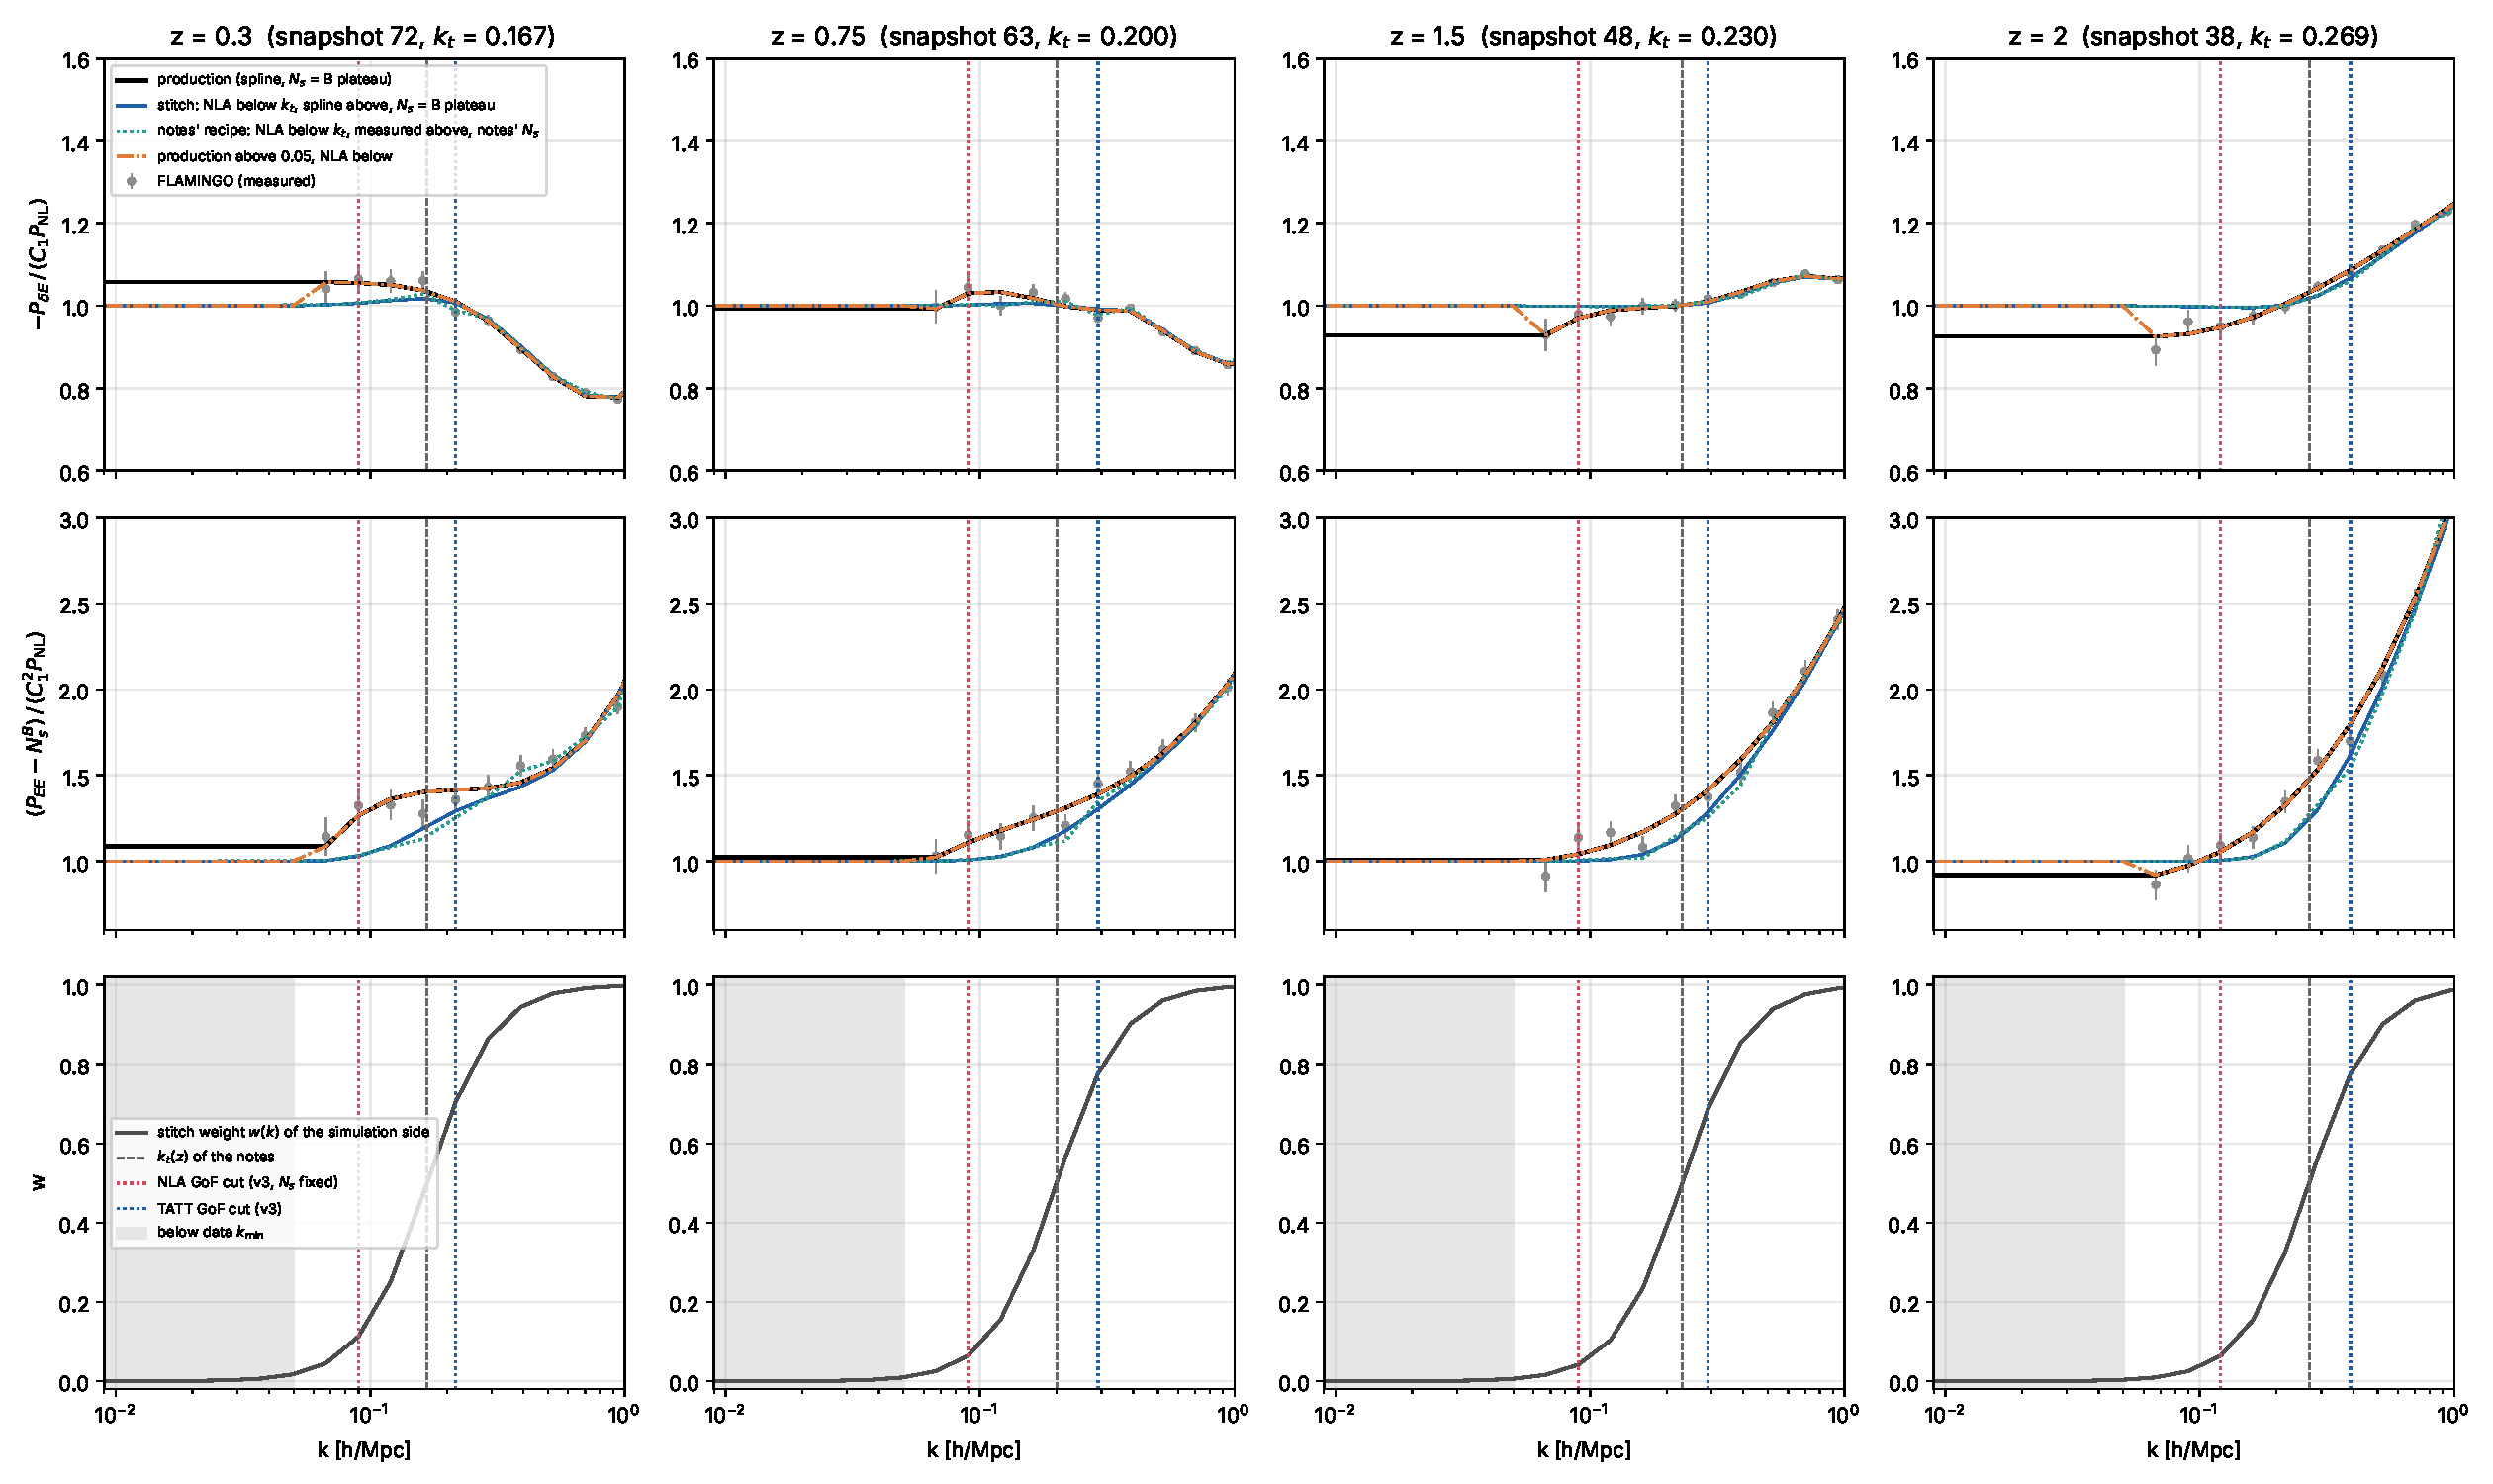
\includegraphics[width=\textwidth]{fig_stitch_truths}
\caption{Production and stitched truths against the measured FLAMINGO ratios,
normalised to the notes' NLA side, for four core snapshots (GI top, II
middle, stitch weight bottom). Grey dashed: $k_t(z)$; red and blue dotted:
the $k_{\max}$ at which the production-truth goodness of fit rejects NLA and
TATT. Between the red line and $k_t$ the stitch replaces a measured
departure from NLA by NLA.}
\end{figure}

\section{Goodness of fit versus $k_{\max}$}

\begin{figure}[H]
\centering
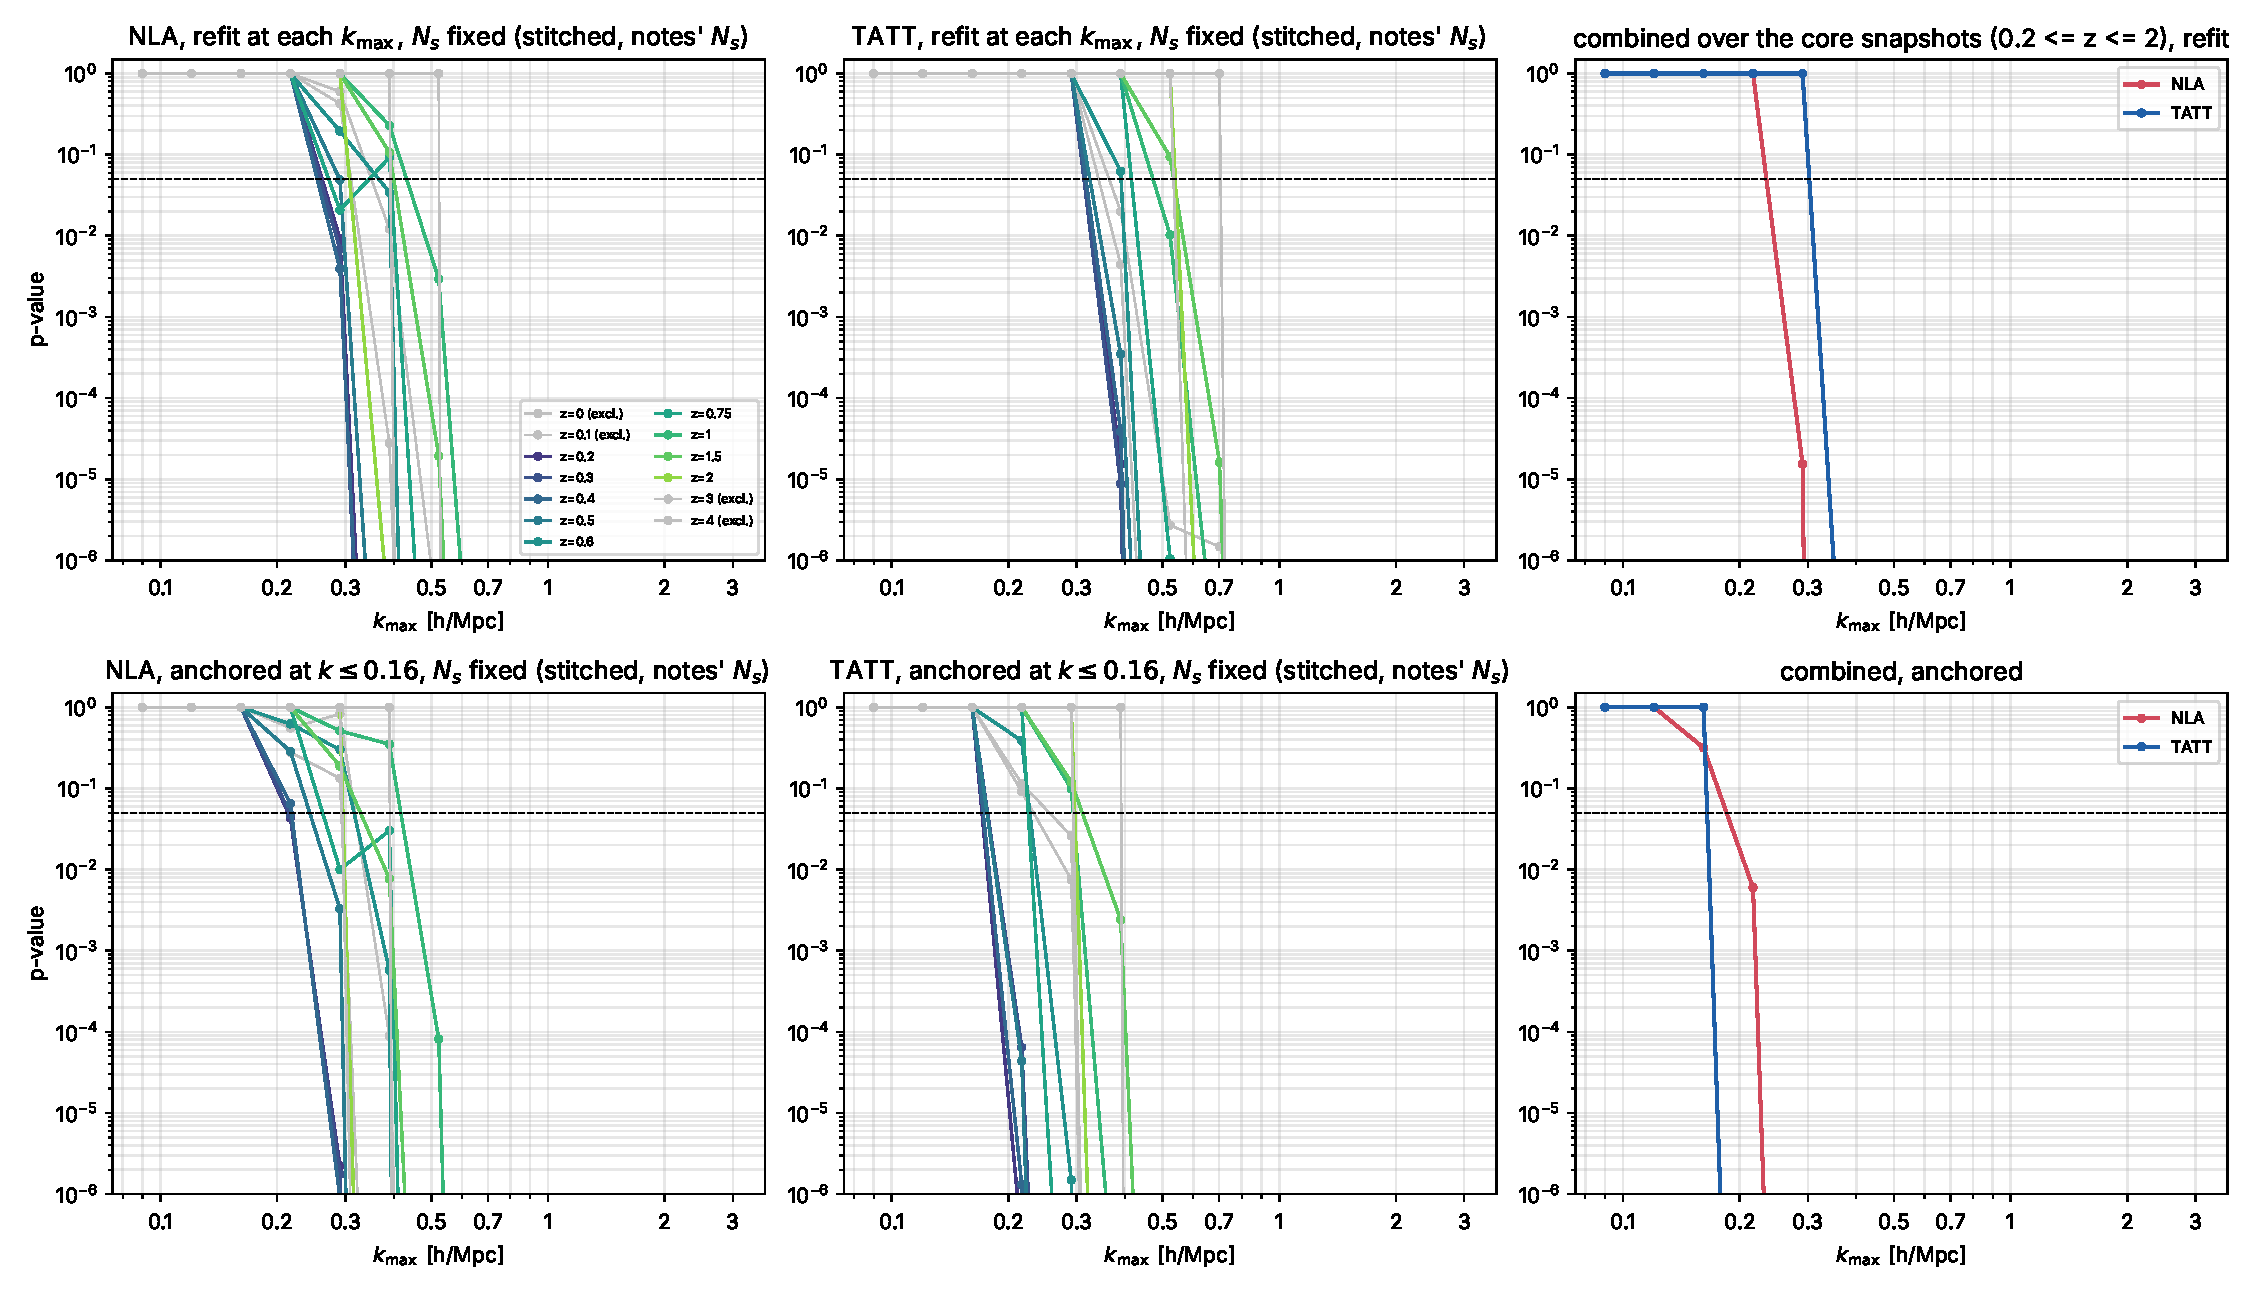
\includegraphics[width=\textwidth]{fig_v3_gof}
\caption{Stitched truth (S2). Top: $p$-value of the refit at each
$k_{\max}$ per snapshot (colour: core snapshots) and combined over the core.
Bottom: anchored at $k \le 0.16$. Plateaus at $p = 1$ are the no-test regime
(effective dof below one).}
\end{figure}

\subsection{Refit}
NLA passes to 0.22$\hmpc$ at $z \le 0.5$ and to 0.29 to 0.39 at $0.6 \le z
\le 1.5$, failing at the next grid step with $p \sim 10^{-2}$ to $10^{-5}$;
the combined core $p$ is 1 at 0.22 and $1.5\times 10^{-5}$ at 0.29. TATT
passes to 0.29 at $z \le 0.5$ (where no test is possible before 0.39) and to
0.39 to 0.52 at higher $z$; combined $p$ = 1 at 0.29, $3\times 10^{-10}$ at
0.39. In units of the transition scale the NLA cut is 1.2 to 1.35 $k_t$ at
$z \le 0.5$, 1.7 to 1.95 $k_t$ at $z$ = 0.75 to 1.5 and 1.1 $k_t$ at $z = 2$.

\subsection{Anchored: not meaningful for TATT here}
The anchored criterion fixes the parameters by the fit to $k \le 0.16$ and
scores the extrapolation. On the stitched truth $k \le 0.16$ is almost pure
NLA ($w \le 0.5$ at $z \le 0.5$, $w \le 0.3$ at $z \ge 0.75$), so the anchor
carries no information on $A_2$ and $b_{\rm TA}$: the anchor fits give $A_2
= -0.2 \pm 0.5$ to $0.1 \pm 2.3$ ($0 \pm 6$ at $z = 1.5$) and $b_{\rm TA} =
0.1 \pm 0.2$ to $0 \pm 2.5$. Extrapolating those values into 0.16 to 0.22,
where the simulation side has weight, gives $p$ = $10^{-7}$ to $4\times
10^{-5}$ at $z$ = 0.2 to 0.5 and the combined TATT curve fails at 0.22, below
NLA (0.29), whose single parameter the noise-free NLA side pins exactly.
This is a property of the anchor, not of TATT; the anchored TATT cuts are
listed but not used.

\section{Redshift-dependent cuts}

\begin{figure}[H]
\centering
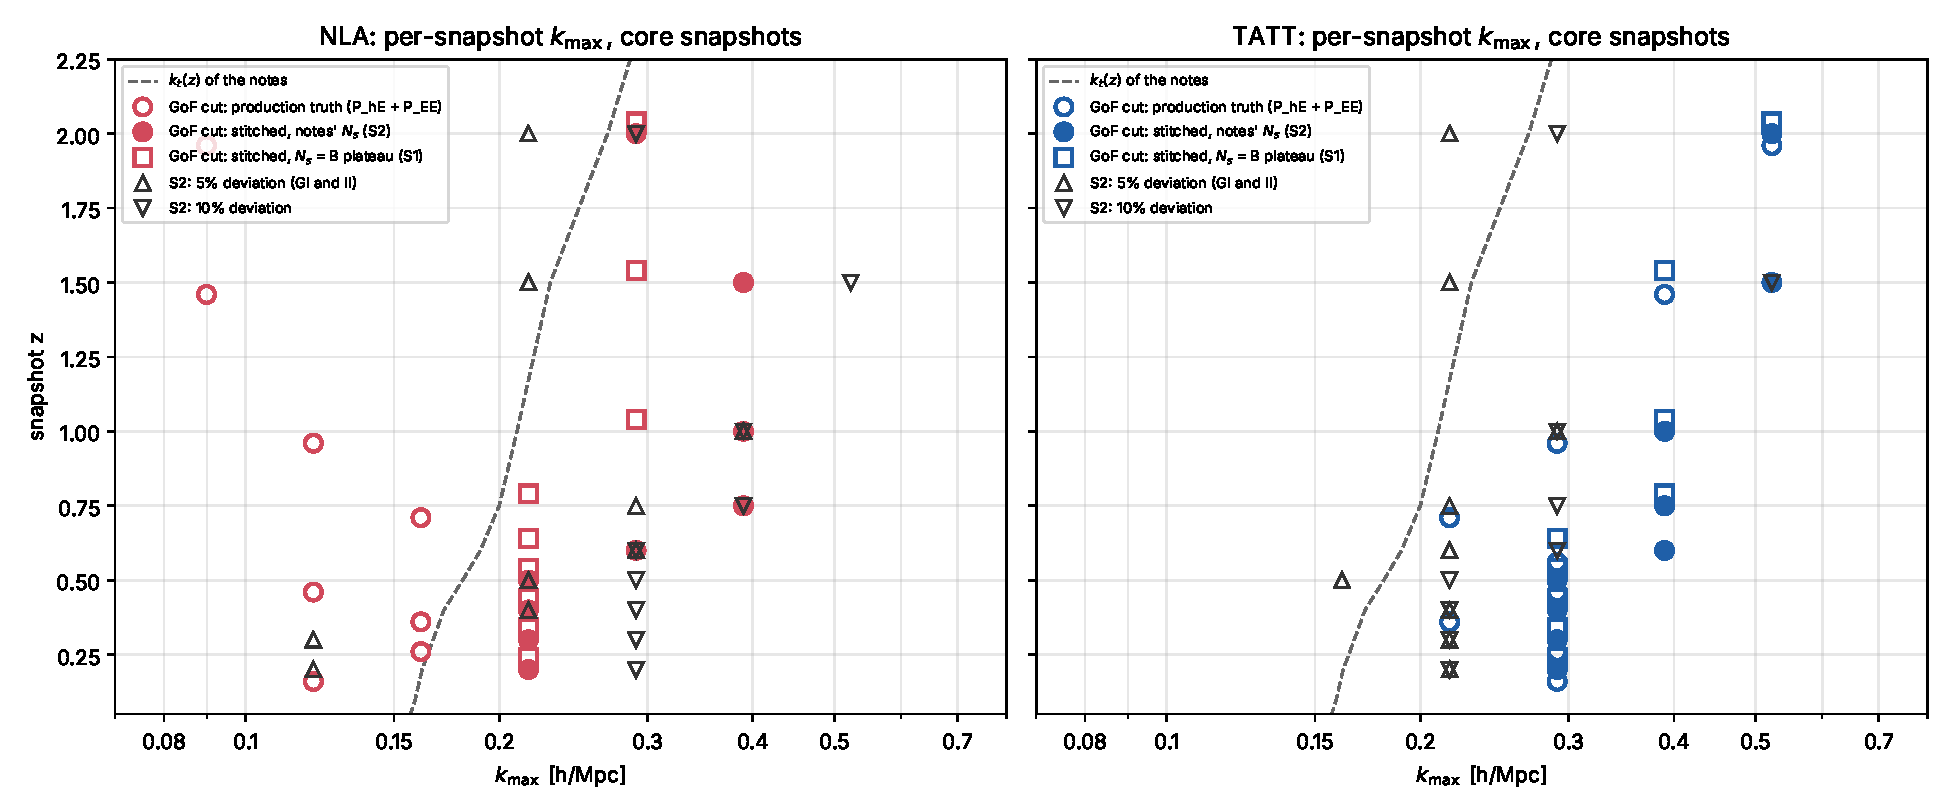
\includegraphics[width=\textwidth]{fig_s_cuts}
\caption{Per-snapshot cuts, core snapshots ($k$ horizontal, $z$ vertical).
Filled: refit GoF on the stitched truth (S2); open circles: the same on the
production truth with the same two probes; open squares: S1 (B-plateau
$N_s$); triangles: 5 and 10 per cent deviation of the anchored model from
the stitched truth. Dashed: $k_t(z)$.}
\end{figure}

\begin{table}[H]
\centering\footnotesize
\setlength{\tabcolsep}{4pt}
\caption{Cuts in $h$/Mpc on the $k_{\max}$ grid (0.09, 0.12, 0.16, 0.22,
0.29, 0.39, 0.52, 0.70, \dots), core snapshots. GoF: refit, two
consecutive $p<0.05$; 5\% and 10\%: anchored model within that fraction of
the noise-free truth on both GI and II. ``nan'': fails at the first grid
step.}
\label{tab:cuts}
\begin{tabular}{cc|cccc|cccc|cc}
\toprule
 & & \multicolumn{4}{c|}{NLA, stitched (S2)} & \multicolumn{4}{c|}{TATT, stitched (S2)} & \multicolumn{2}{c}{production GoF} \\
$z$ & $k_t$ & GoF & anch. & 5\% & 10\% & GoF & anch. & 5\% & 10\% & NLA & TATT \\
\midrule
0.2 & 0.162 & 0.22 & 0.16 & 0.12 & 0.29 & 0.29 & 0.16 & 0.22 & 0.22 & 0.12 & 0.29 \\
0.3 & 0.167 & 0.22 & 0.16 & 0.12 & 0.29 & 0.29 & 0.16 & 0.22 & 0.22 & 0.16 & 0.29 \\
0.4 & 0.172 & 0.22 & 0.22 & 0.22 & 0.29 & 0.29 & 0.16 & 0.22 & 0.22 & 0.16 & 0.22 \\
0.5 & 0.181 & 0.22 & 0.22 & 0.22 & 0.29 & 0.29 & 0.16 & 0.16 & 0.22 & 0.12 & 0.29 \\
0.6 & 0.190 & 0.29 & 0.29 & 0.29 & 0.29 & 0.39 & 0.22 & 0.22 & 0.29 & -- & 0.29 \\
0.75 & 0.200 & 0.39 & 0.22 & 0.29 & 0.39 & 0.39 & 0.22 & 0.22 & 0.29 & 0.16 & 0.22 \\
1 & 0.210 & 0.39 & 0.39 & 0.39 & 0.39 & 0.39 & 0.29 & 0.29 & 0.29 & 0.12 & 0.29 \\
1.5 & 0.230 & 0.39 & 0.29 & 0.22 & 0.52 & 0.52 & 0.29 & 0.22 & 0.52 & 0.09 & 0.39 \\
2 & 0.269 & 0.29 & 0.29 & 0.22 & 0.29 & 0.52 & 0.29 & 0.22 & 0.29 & 0.09 & 0.52 \\
\bottomrule
\end{tabular}
\end{table}

\begin{figure}[H]
\centering
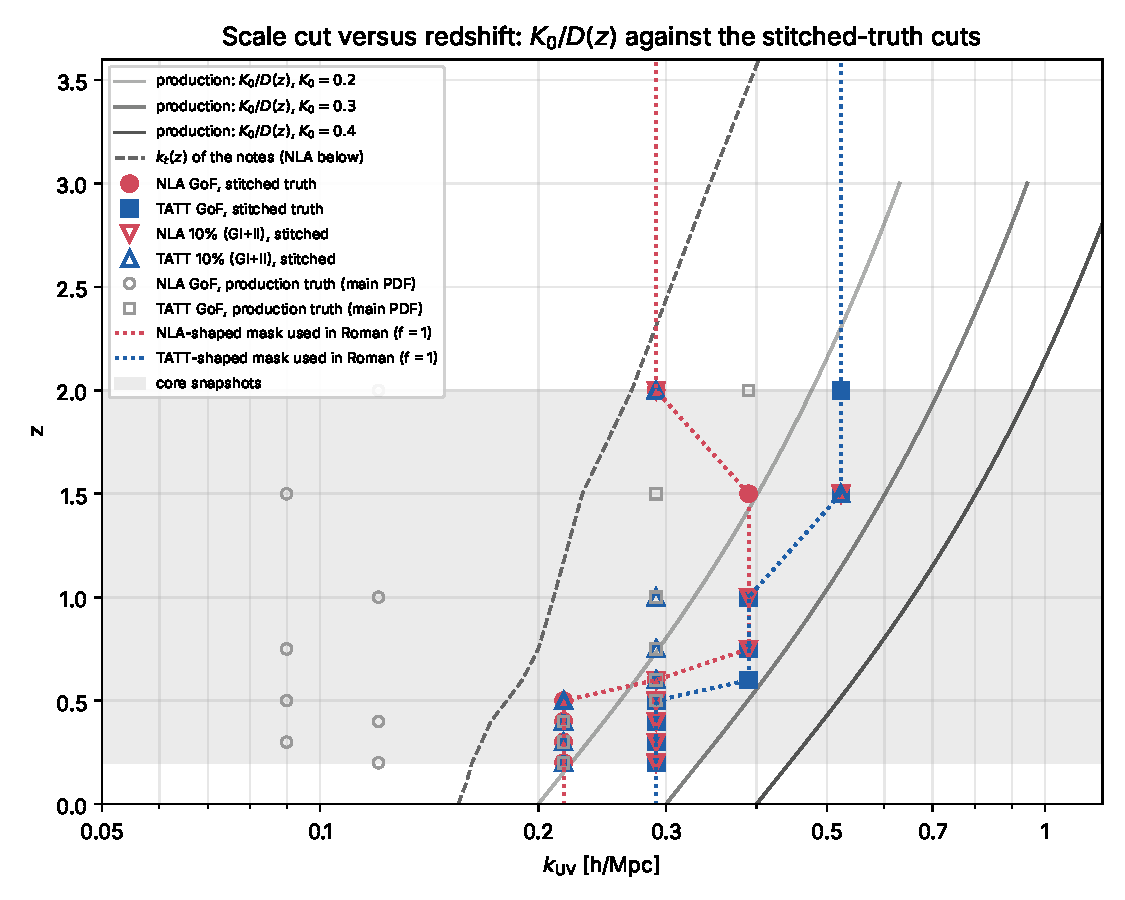
\includegraphics[width=0.78\textwidth]{fig_s_kuv_z}
\caption{$k_{\rm UV}(z)$: the production $K_0/D(z)$ family (grey curves),
$k_t(z)$ (dashed), the stitched-truth cuts (filled: GoF; open: 10 per cent)
and the production-truth GoF cuts (small grey). Dotted: the redshift-dependent
masks used in Roman (Section 6).}
\end{figure}

The stitched-truth cuts rise with redshift, as $k_t(z)$ does (factor 1.7
from $z = 0.2$ to 2): TATT by a factor 1.8, NLA by 1.3 with a peak of 0.39
at $z$ = 0.75 to 1.5. The production cuts are flat or falling in $z$, and
the $K_0/D(z)$ family rises by a factor 2.2 across the core. Expressed as an
equivalent $K_0$, the stitched TATT cut is $K_0 \approx 0.22$ to 0.25 at
every core redshift; the NLA cut is $K_0 \approx 0.25$ at $z \le 1$ and
0.12 at $z = 2$.

\section{$\dchi^2_{\rm FL}$ and its translation to Roman}

\begin{figure}[H]
\centering
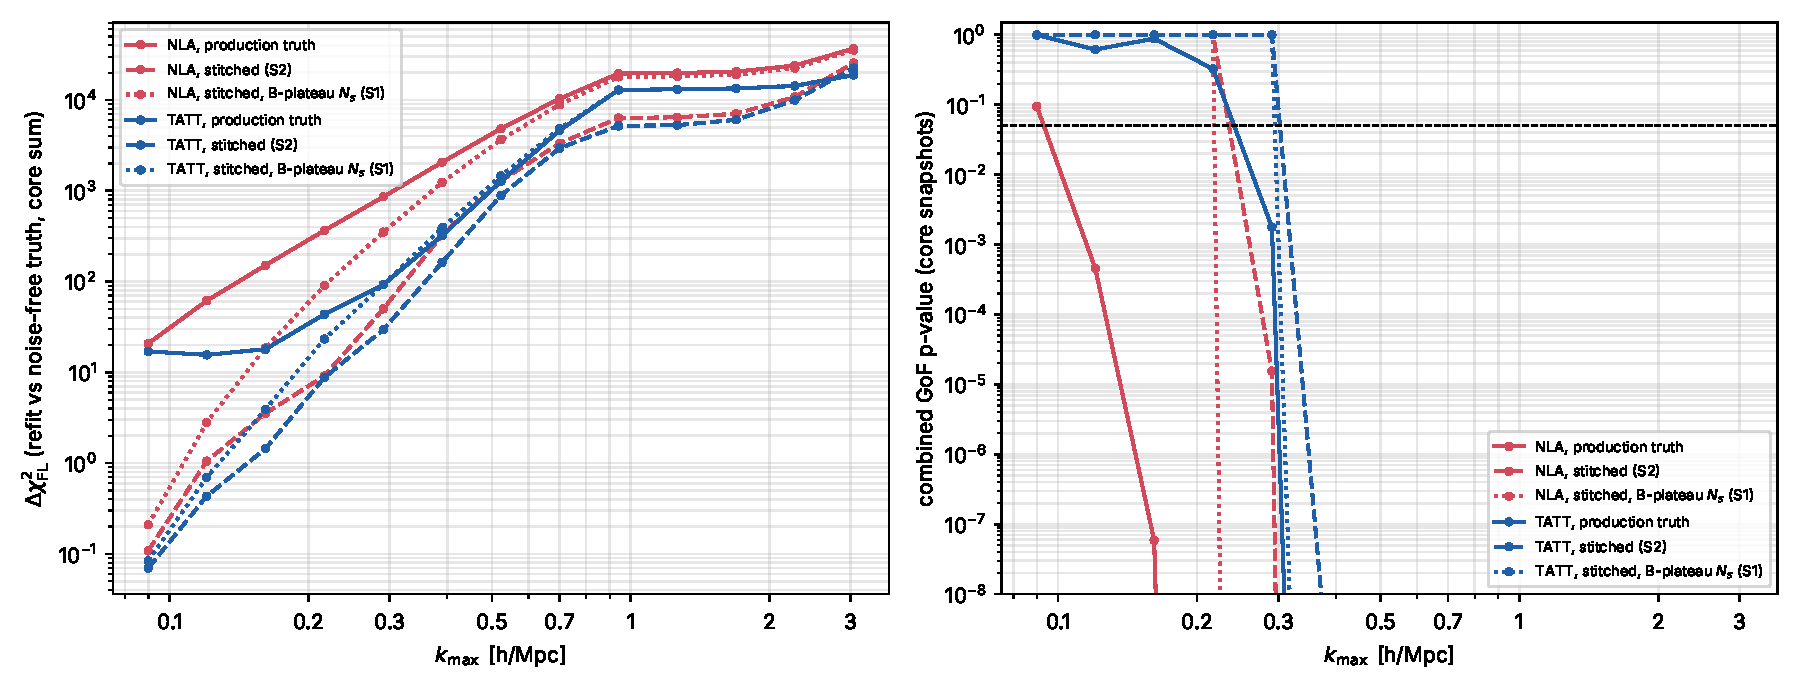
\includegraphics[width=\textwidth]{fig_s_dchi2}
\caption{Left: $\dchi^2_{\rm FL}(k_{\max})$ of the refit against the
noise-free truth, summed over the core snapshots, for the production truth
and the two stitched variants. Right: combined refit $p$-value.}
\end{figure}

On the stitched truth $\dchi^2_{\rm FL}$ starts from zero and both models
track each other up to $k_{\max} \approx 0.3$ (NLA 9.1, TATT 8.8 at 0.22;
50 against 30 at 0.29; 327 against 163 at 0.39), because below $k_t$ both
reproduce the NLA side exactly and the difference between them is the
$A_2$, $b_{\rm TA}$ freedom in the transition. With the production truth
NLA carries 20 at $k_{\max} = 0.09$ already (the white II excess and the
large-scale $A_2$ signal) and TATT 17, falling to 16 at 0.12 as its
parameters lock in.

The translation to Roman uses the same mechanism as the main summary, here
directly: the model with the per-snapshot refit amplitudes at $k_{\max} =
f\times{\rm cut}(z_s)$ is pushed through the sim\_IA tables and compared with
the truth on the Roman mask (right panel of Figure 7). On the TATT-shaped
mask at $f = 1$ the Roman $\dchi^2$ is 1.1 (NLA) / 0.6 (TATT); at $f = 1.4$
it is 6.9 / 3.3, at $f = 2$ 22 / 5.6. On the NLA-shaped mask at $f = 1$ it is
0.04 for both.

\section{Amplitude evolution}

\begin{figure}[H]
\centering
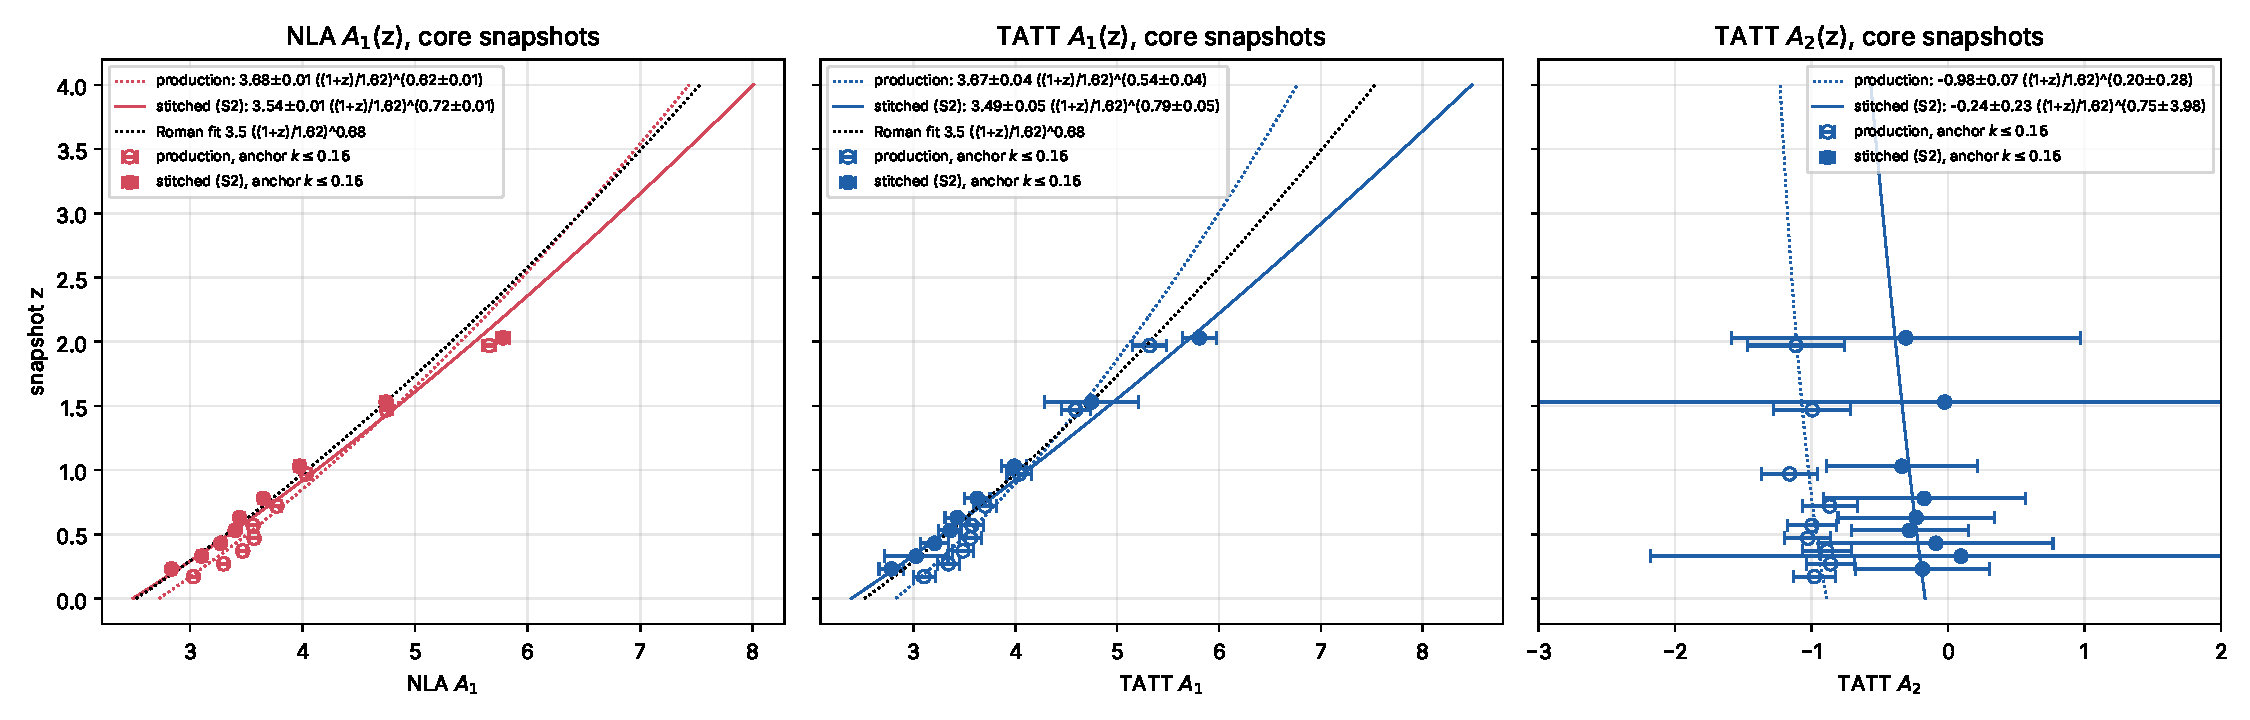
\includegraphics[width=\textwidth]{fig_s_amp}
\caption{$A_1(z)$ (NLA, TATT) and $A_2(z)$ (TATT) at the anchor $k \le 0.16$,
core snapshots, production truth (open) and stitched truth (filled), with
power-law fits $A\,[(1+z)/1.62]^\eta$ and the Roman chain fit.}
\end{figure}

NLA: $A_1 = (3.54 \pm 0.01)\,x^{0.72 \pm 0.01}$ on the stitched truth against
$(3.68 \pm 0.01)\,x^{0.62 \pm 0.01}$ on the production truth, $x =
(1+z)/1.62$; the stitched values are the notes' per-snapshot NLA amplitudes
(the production anchor amplitudes are 1.5 to 7 per cent higher at $z \le 1$
because the white excess and the $A_2$ term are absorbed into $a_1$ when
$N_s$ is fixed to the B plateau). TATT: $A_1 = (3.49 \pm 0.05)\,x^{0.79 \pm
0.05}$; $A_2$ is unconstrained at the anchor ($-0.24 \pm 0.23$ with
$\eta_2 = 0.8 \pm 4$) and $-0.1$ to $-0.3$ with $b_{\rm TA} = 0$ at the cut,
against $A_2 = (-0.98 \pm 0.07)\,x^{0.20 \pm 0.28}$ at the anchor and $-1.3$
at the cut on the production truth. On the stitched truth TATT is NLA plus a
small correction; the tidal-torquing signature of FLAMINGO is a large-scale
one.

\section{Roman: figure of bias on the stitched-truth masks}

The redshift-dependent masks follow the recipe of the main summary:
$k_{\rm UV}(z)$ = the per-snapshot GoF cut of Table~\ref{tab:cuts}
interpolated in $\ln k$ over the core (flat outside) times a factor $f$,
IR/UV masks with the GG + NLA baseline and $\alpha = 0.05$. Data = GG +
stitched truth; model = native NLA / TATT with power-law evolution,
$\Omega_m$ and $A_s$ free (bias\_v2 fit, IA bounded to the chain priors, IA
marginalised at the flat-prior width), Gaussian covariance; the FoB
uncertainty propagates the simulation's error bars weighted by $w(k)$.

\begin{figure}[H]
\centering
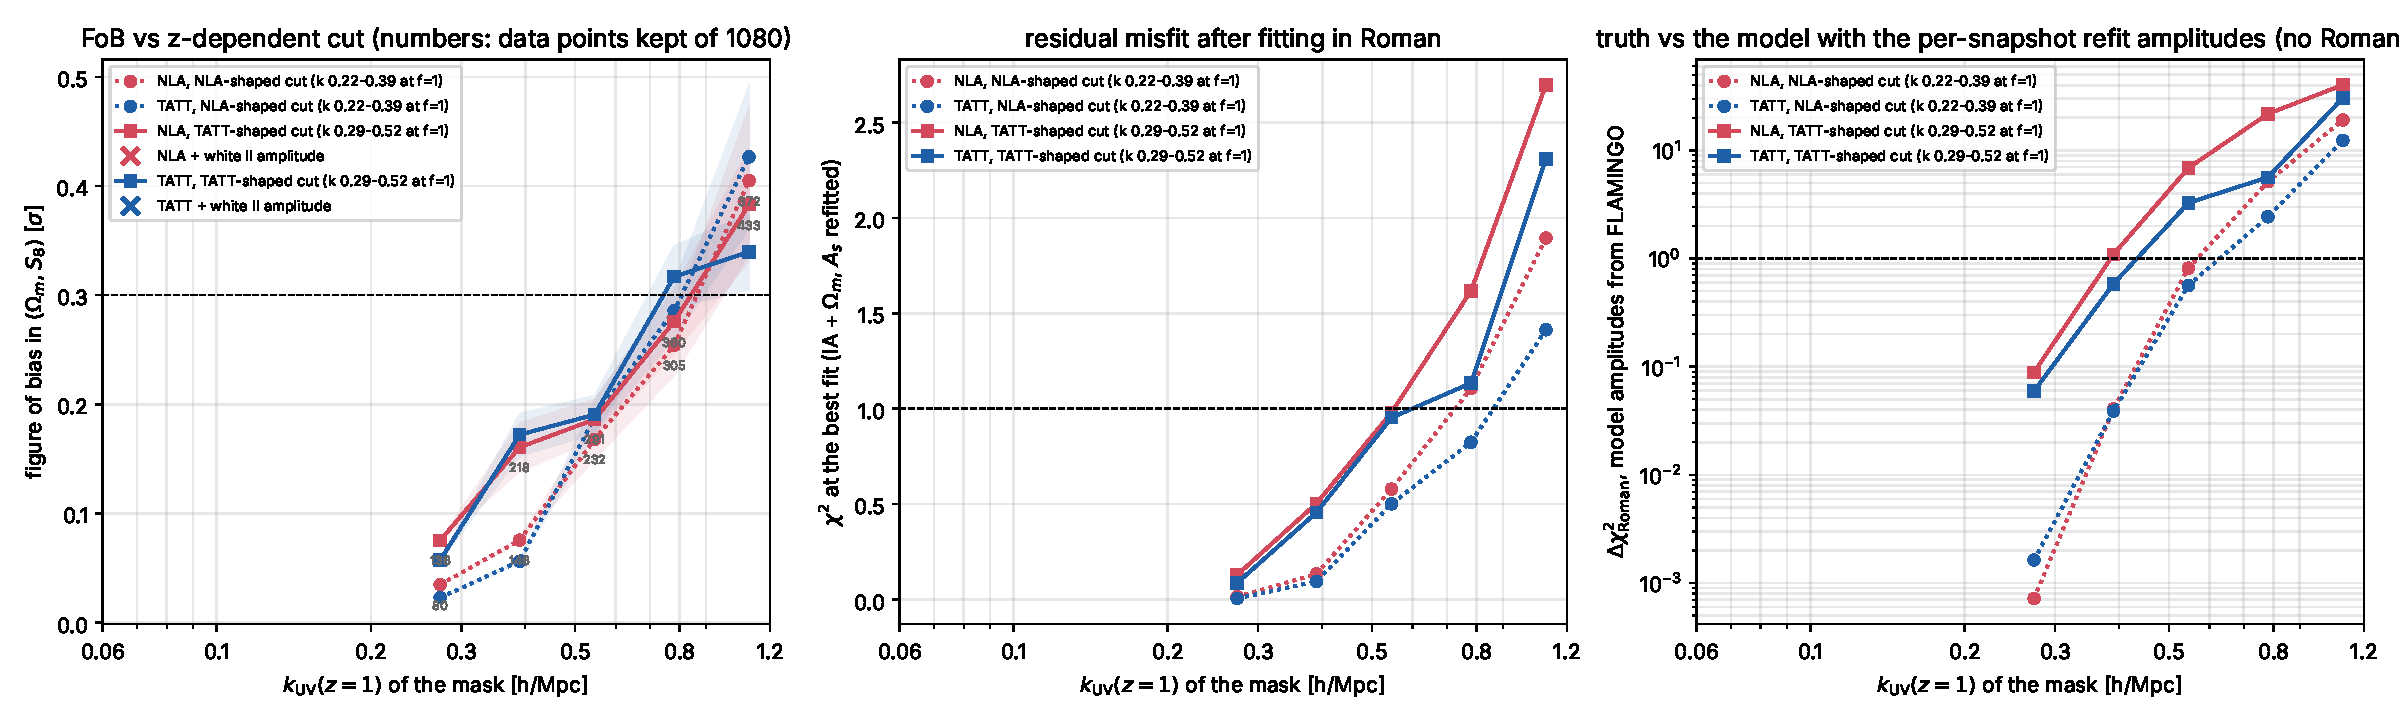
\includegraphics[width=\textwidth]{fig_v3_roman}
\caption{Stitched truth. Left: FoB in $(\Omega_m, S_8)$ against the mask
(labelled by $k_{\rm UV}$ at $z = 1$; numbers: data points kept of 1080),
NLA-shaped (dotted) and TATT-shaped (solid) cuts times $f$ = 0.7, 1, 1.4, 2,
2.8. Middle: best-fit $\chi^2$. Right: Roman $\dchi^2$ of the truth against
the model with the per-snapshot refit amplitudes (no Roman refit).}
\end{figure}

\begin{table}[H]
\centering\footnotesize
\caption{Roman results on the stitched-truth masks (NLA / TATT fitted).}
\begin{tabular}{lcccrccc}
\toprule
mask shape & $f$ & $k_{\rm UV}(z{=}0.5)$ & $k_{\rm UV}(z{=}1)$ & points & $\dchi^2_{\rm Roman}$ & $\chi^2$ best fit & FoB \\
\midrule
NLA-shaped & 0.7 & 0.15 & 0.27 & 80 & 0.00 / 0.00 & 0.01 / 0.01 & 0.03 / 0.02 $\pm$ 0.00 \\
NLA-shaped & 1 & 0.22 & 0.39 & 146 & 0.04 / 0.04 & 0.13 / 0.10 & 0.08 / 0.06 $\pm$ 0.00 \\
NLA-shaped & 1.4 & 0.31 & 0.55 & 232 & 0.82 / 0.56 & 0.58 / 0.50 & 0.17 / 0.19 $\pm$ 0.02 \\
NLA-shaped & 2 & 0.44 & 0.78 & 305 & 5.13 / 2.43 & 1.11 / 0.82 & 0.25 / 0.29 $\pm$ 0.03 \\
NLA-shaped & 2.8 & 0.62 & 1.09 & 372 & 19.09 / 12.38 & 1.89 / 1.41 & 0.40 / 0.43 $\pm$ 0.07 \\
TATT-shaped & 0.7 & 0.21 & 0.27 & 136 & 0.09 / 0.06 & 0.13 / 0.09 & 0.08 / 0.06 $\pm$ 0.00 \\
TATT-shaped & 1 & 0.30 & 0.39 & 218 & 1.09 / 0.58 & 0.50 / 0.46 & 0.16 / 0.17 $\pm$ 0.02 \\
TATT-shaped & 1.4 & 0.42 & 0.55 & 291 & 6.88 / 3.27 & 0.98 / 0.95 & 0.19 / 0.19 $\pm$ 0.02 \\
TATT-shaped & 2 & 0.59 & 0.78 & 360 & 21.76 / 5.64 & 1.62 / 1.13 & 0.28 / 0.32 $\pm$ 0.03 \\
TATT-shaped & 2.8 & 0.83 & 1.09 & 433 & 40.31 / 30.58 & 2.70 / 2.31 & 0.38 / 0.34 $\pm$ 0.04 \\
\bottomrule
\end{tabular}
\end{table}

Both models are well inside the criterion on their own cuts: FoB 0.08 /
0.06 on the NLA-shaped mask and 0.16 / 0.17 on the TATT-shaped mask, with
$\chi^2$ of 0.1 and 0.5. $\chi^2 = 1$ is reached at $1.4\times$ the TATT cut
($k_{\rm UV}(z{=}1) = 0.55$) and FoB = 0.3 at about $2\times$ (0.78), for
either model. For comparison, on the production truth the TATT-shaped mask
at $f = 1$ (0.22 to 0.29) gives 0.23 / 0.22 and FoB = 0.3 is crossed at
$f \approx 1.3$.

\section{Roman test with all parameters free, $K_0/D(z)$ masks}

This section is the earlier supplement, kept for reference: the stitched
truths through the Section 8 machinery of the main summary (every parameter
free, case A: $\Omega_m, A_s$; case B adds $n_s, H_0, \Omega_b$ with the
chain priors), on the production $K_0/D(z)$ masks and the flat TATT-shaped
cuts of the \emph{production} analysis. Variants there: S1 and S2 as above
(spline simulation side); S3 = the notes' recipe with the measured
simulation side; S4 = production above $k = 0.05$ and NLA below.

\begin{figure}[H]
\centering
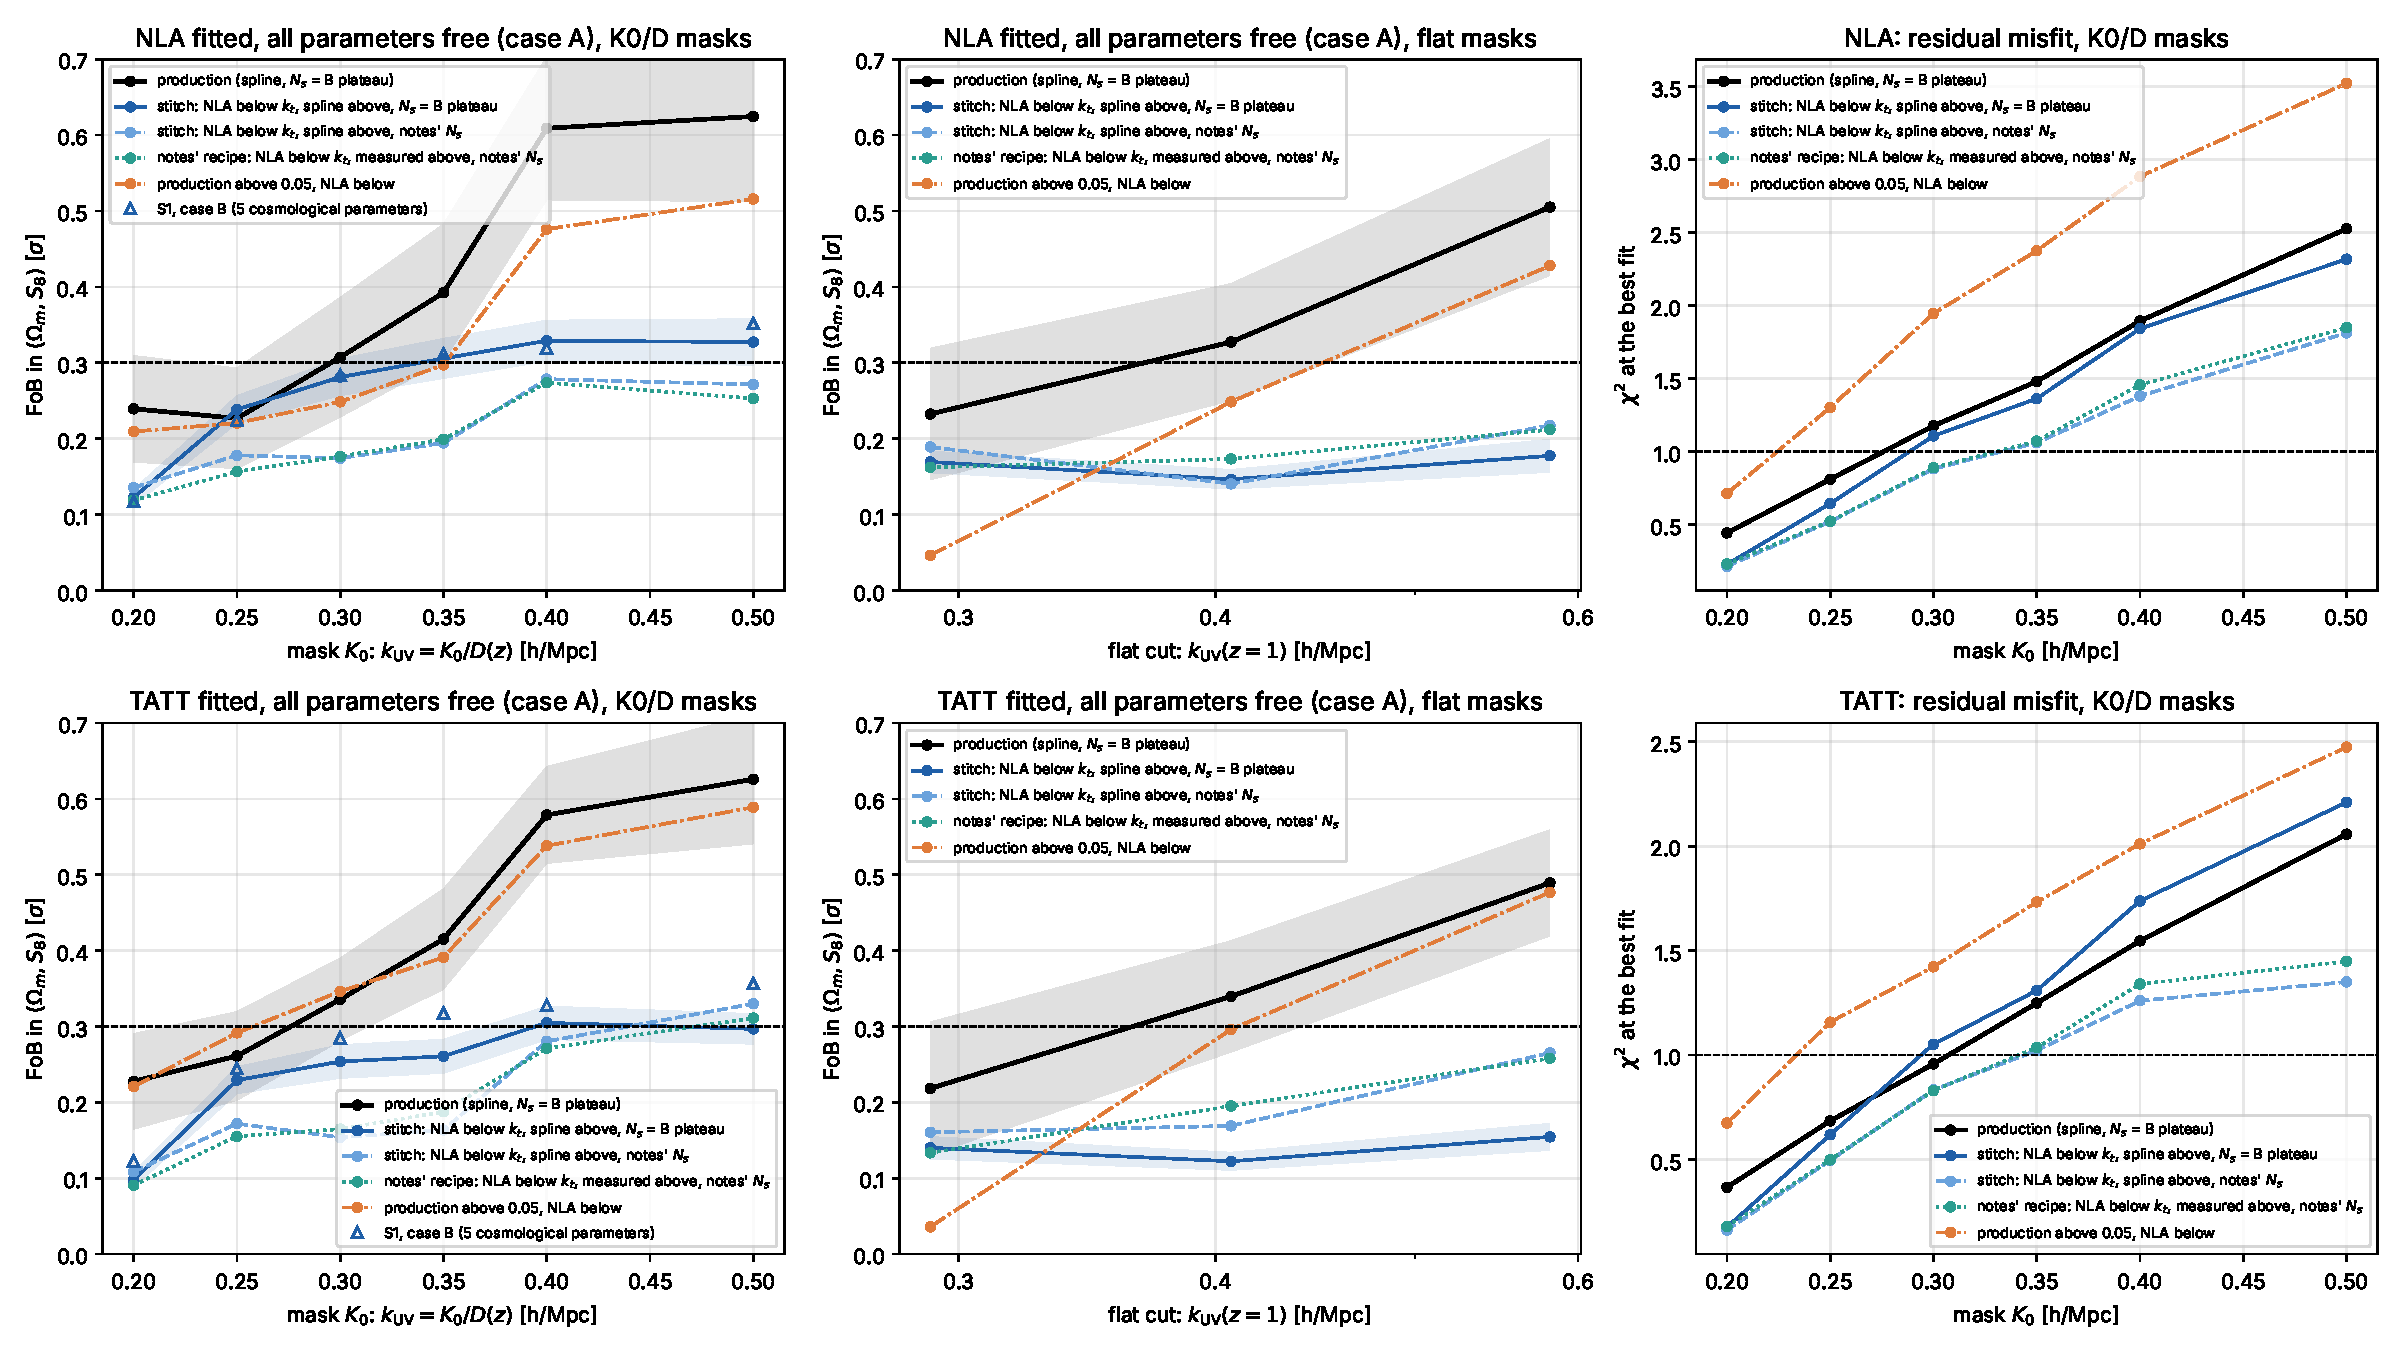
\includegraphics[width=\textwidth]{fig_stitch_fob}
\caption{FoB (left, middle) and best-fit $\chi^2$ (right) against the cut
for the production truth (black) and the stitched variants, NLA fitted
(top) and TATT fitted (bottom), case A; open triangles: S1 in case B.}
\end{figure}

\begin{figure}[H]
\centering
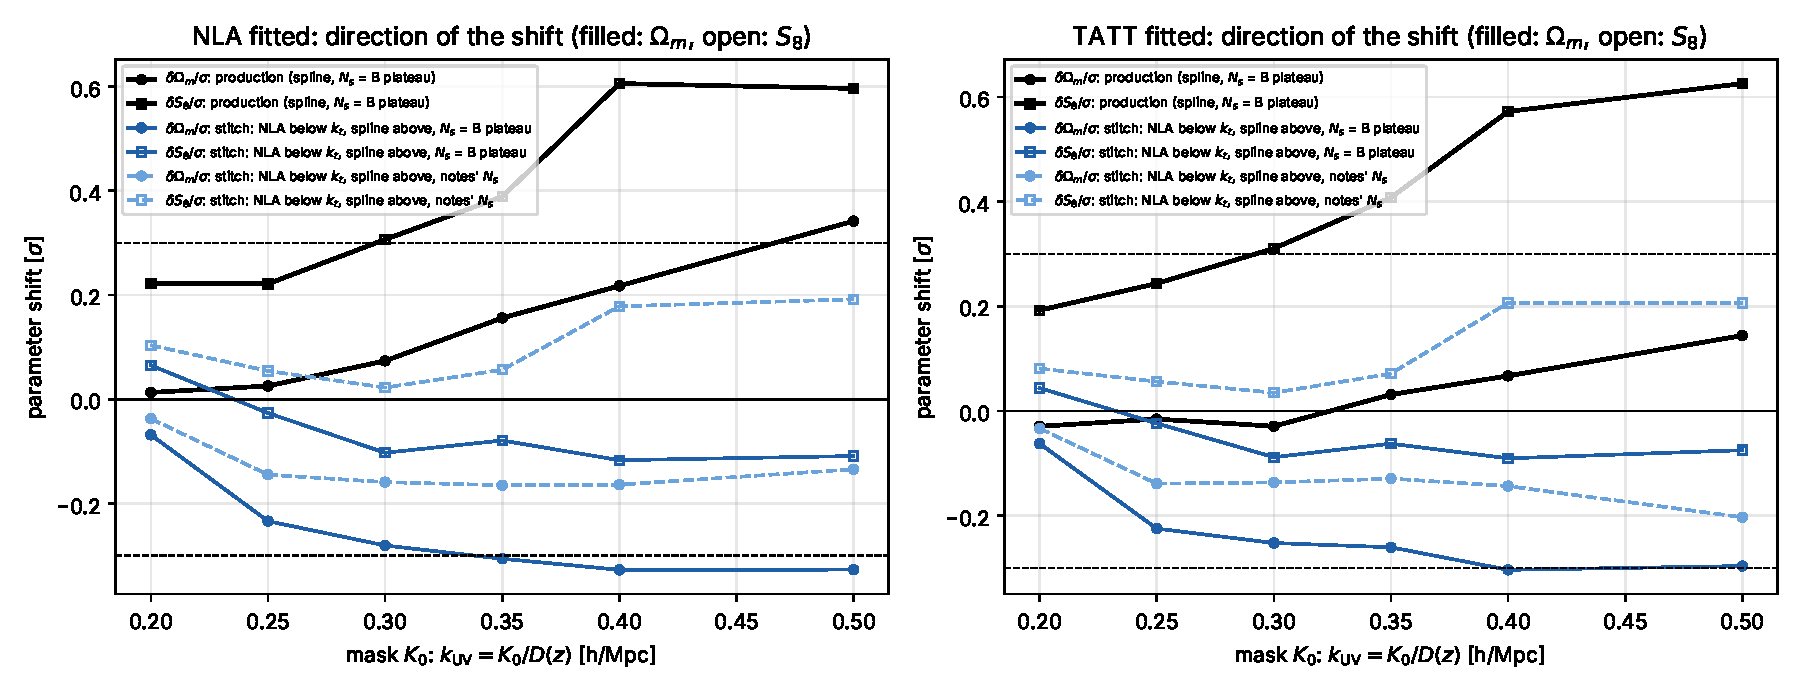
\includegraphics[width=\textwidth]{fig_stitch_shift}
\caption{$\delta\Omega_m/\sigma$ (filled) and $\delta S_8/\sigma$ (open)
against $K_0$ for the production truth and the stitched variants S1, S2.}
\end{figure}

\begin{table}[H]
\centering\footnotesize
\setlength{\tabcolsep}{4pt}
\caption{Case A, $K_0/D(z)$ masks: FoB (NLA / TATT), best-fit $\chi^2$ in
brackets, and $\dchi^2_{\rm Roman}$ of each variant against the production
truth on the same mask.}
\label{tab:stitch}
\resizebox{\textwidth}{!}{%
\begin{tabular}{lcccccc}
\toprule
$K_0$ [$h$/Mpc] & 0.2 & 0.25 & 0.3 & 0.35 & 0.4 & 0.5 \\
\midrule
production & 0.24 / 0.23 [0.44 / 0.37] & 0.23 / 0.26 [0.81 / 0.69] & 0.31 / 0.34 [1.18 / 0.96] & 0.39 / 0.41 [1.48 / 1.25] & 0.61 / 0.58 [1.90 / 1.55] & 0.62 / 0.63 [2.53 / 2.06] \\
S2 stitch, notes' $N_s$ & 0.14 / 0.11 [0.21 / 0.16] & 0.18 / 0.17 [0.52 / 0.50] & 0.17 / 0.15 [0.88 / 0.83] & 0.19 / 0.16 [1.06 / 1.02] & 0.28 / 0.28 [1.38 / 1.26] & 0.27 / 0.33 [1.81 / 1.35] \\
S1 stitch, $N_s^B$ & 0.12 / 0.10 [0.23 / 0.18] & 0.24 / 0.23 [0.65 / 0.62] & 0.28 / 0.25 [1.11 / 1.05] & 0.31 / 0.26 [1.36 / 1.31] & 0.33 / 0.30 [1.84 / 1.74] & 0.33 / 0.30 [2.32 / 2.21] \\
S3 notes literal & 0.12 / 0.09 [0.23 / 0.18] & 0.16 / 0.15 [0.52 / 0.50] & 0.18 / 0.17 [0.89 / 0.83] & 0.20 / 0.19 [1.07 / 1.04] & 0.27 / 0.27 [1.46 / 1.34] & 0.25 / 0.31 [1.85 / 1.45] \\
S4 NLA below 0.05 & 0.21 / 0.22 [0.71 / 0.68] & 0.22 / 0.29 [1.30 / 1.16] & 0.25 / 0.35 [1.95 / 1.42] & 0.30 / 0.39 [2.38 / 1.73] & 0.48 / 0.54 [2.88 / 2.01] & 0.52 / 0.59 [3.52 / 2.47] \\
\midrule
$\dchi^2_{\rm Roman}$(S2 $-$ prod) & 2.4 & 3.1 & 3.5 & 3.8 & 4.2 & 4.7 \\
$\dchi^2_{\rm Roman}$(S1 $-$ prod) & 2.3 & 2.9 & 3.3 & 3.6 & 4.2 & 4.8 \\
$\dchi^2_{\rm Roman}$(S3 $-$ prod) & 2.3 & 3.1 & 3.6 & 3.9 & 4.4 & 4.9 \\
$\dchi^2_{\rm Roman}$(S4 $-$ prod) & 1.1 & 1.3 & 1.5 & 1.5 & 1.6 & 1.6 \\
\bottomrule
\end{tabular}}
\end{table}

\paragraph{Reading.} With the notes' $N_s$ (S2, S3) the FoB stays at 0.11 to
0.19 up to $K_0 = 0.35$ and reaches 0.28 at $K_0 = 0.4$; with the B-plateau
$N_s$ (S1) it crosses 0.3 at $K_0 \approx 0.34$ (NLA) / 0.39 (TATT). The
best-fit $\chi^2$ barely moves between production and S1 (1.18 / 0.96 against
1.11 / 1.05 at $K_0 = 0.3$): nearly all of the residual misfit lives above
$k_t$. What changes is the direction of the shift: the production truth
biases $S_8$ (+0.3 to +0.6$\sigma$, growing with $K_0$ through the white II
excess, which enters $\xi_-$ as $\theta^{-2}$ and no $k$ mask removes), the
stitched truth biases $\Omega_m$ ($-0.3\sigma$, saturating for $K_0 \ge
0.35$) through the transition-regime GI/II misfit at $0.2 \lesssim k
\lesssim 1\hmpc$. S3 differs from S2 by at most 0.03 (the FLAMINGO noise
above $k_t$ is not what drives this); case B differs from case A by $-0.01$
to $+0.06$. S4's hard join at 0.05 raises $\chi^2$ by 0.3 to 1.0 and moves
the FoB by at most 0.05; the smooth version of that extrapolation (white
term kept white below 0.05, \texttt{bias\_phys.py}) changes the production
FoB by less than 0.02.

\section{Code}
\begin{itemize}\sloppy
\item \texttt{v3/v3\_flamingo.py}: the v3 analysis, now callable with a
  \texttt{truth} dictionary (data, truth, $N_s$, weights, probes, output
  directory); \texttt{pvalue()} is the weighted (Satterthwaite) test. The
  default run reproduces the stored v3 results exactly (checked).
\item \texttt{v3s/run\_stitched.py}: builds the S2, S1, S2w and prod2 truths
  and runs \texttt{v3\_flamingo.main} into \texttt{v3s/\{S2,S1,S2w,prod2\}/}
  (\texttt{v3.npz}, \texttt{cuts.csv}, \texttt{combined.csv},
  \texttt{amplitudes.csv}, \texttt{summary.json}, figures
  \texttt{fig\_v3\_*}).
\item \texttt{v3s/plot\_stitched\_cuts.py}: \texttt{fig\_s\_cuts},
  \texttt{fig\_s\_kuv\_z}, \texttt{fig\_s\_dchi2}, \texttt{fig\_s\_amp},
  \texttt{cuts\_compare.csv}.
\item \texttt{v3/v3\_roman.py} (options \texttt{--fits-dir}, \texttt{--truth},
  \texttt{--out}, \texttt{--stitched}): masks from the stitched cuts, Roman
  $\dchi^2$ and FoB; \texttt{v3/plot\_v3\_roman.py} run in
  \texttt{v3s/S2/} for \texttt{fig\_v3\_roman}, \texttt{roman\_results.csv}.
\item \texttt{v3/stitched\_test.py}, \texttt{v3/plot\_stitched.py}: Section 7
  (\texttt{stitched\_truths.npz}, \texttt{stitched\_xi.npz},
  \texttt{stitched\_test.json/.csv}, \texttt{fig\_stitch\_*}).
\item Inputs: \texttt{v2/fits.npz}, \texttt{spectra.npz}
  (\texttt{build\_spectra.py}: notes' $a_1$, $N_s$, stitched ratios),
  \texttt{tatt\_fit/fit\_stitched\_kmax.py} ($k_t$, $w$),
  \texttt{cocoa/run/cosmolike\_xi\_ia.npz},
  \texttt{cocoa/analysis/cov\_gauss\_d3a.npy}, \texttt{J\_cells.npy}.
\end{itemize}
\end{document}
